\section{Experimental Evaluation}
\label{sec:experiments}

We perform a comprehensive empirical evaluation of MABSplit across synthetic and real-world benchmarks to answer the following research questions:
\begin{itemize}
    \item \textbf{RQ1 (Speedup \& Scalability):} Does MABSplit achieve substantial training speedups compared to exact CART and state-of-the-art histogram estimators?
    \item \textbf{RQ2 (Statistical Fidelity):} Does MABSplit preserve exact split choices and test-set generalization accuracy?
    \item \textbf{RQ3 (Ablation Analysis):} What are the individual contributions of Serfling bounds, H-MAB pruning, ADMA allocation, and the Depth-Adaptive Hybrid solver?
    \item \textbf{RQ4 (Ensemble Scaling):} How does MABSplit perform when scaled to Random Forest ensembles?
\end{itemize}

\subsection{Experimental Setup}
\begin{table}[htbp]
\centering
\caption{Benchmark Dataset Summary and Characteristics}
\label{tab:datasets}
\begin{tabular}{lrrrr}
\toprule
\textbf{Dataset} & \textbf{Samples ($N$)} & \textbf{Features ($D$)} & \textbf{Classes ($C$)} & \textbf{Domain} \\
\midrule
Synthetic-100K   & 100,000 & 20  & 2 & Synthetic \\
Synthetic-500K   & 500,000 & 50  & 2 & Synthetic \\
Adult Census     & 48,842  & 14  & 2 & Socioeconomic \\
Covertype        & 581,012 & 54  & 7 & Geospatial \\
HIGGS            & 1,000,000 & 28 & 2 & High-Energy Physics \\
\bottomrule
\end{tabular}
\end{table}


\subsubsection{Datasets}
We evaluate on five standard tabular classification benchmarks summarizing diverse sample scales ($N \in [4.8\times 10^4, 1.0\times 10^6]$) and dimensionality ($D \in [14, 54]$), as detailed in Table~\ref{tab:datasets}. All continuous features are pre-binned into $B=256$ bins.

\subsubsection{Baselines and Hyperparameters}
We benchmark MABSplit against four representative baselines spanning exact, heuristic, and stochastic paradigms:
\begin{enumerate}
    \item \textbf{Scikit-Learn Exact CART} \cite{breiman1984classification}: Standard exact greedy decision tree builder ($\mathcal{O}(D N \log N)$).
    \item \textbf{Extremely Randomized Trees (ExtraTrees)} \cite{geurts2006extremely}: Fast tree induction using random cut thresholds without sorting ($\mathcal{O}(D N)$).
    \item \textbf{Baseline MABSplit} \cite{tiwari2022mabsplit}: The original multi-armed bandit node splitting subroutine relying on naive i.i.d. Hoeffding bounds and static minibatch allocations.
    \item \textbf{HistGradientBoosting} \cite{ke2017lightgbm}: Optimized histogram-based binned gradient booster.
\end{enumerate}
Unless stated otherwise, hyperparameters for single trees are set to $\text{max\_depth} = 12$, $\text{min\_samples\_split} = 10$, $\epsilon = 0.01$, $\delta = 0.05$, $M_0 = 128$, and $N_{\text{thresh}} = 256$. Experiments are repeated over 10 independent random seeds.

\subsection{Benchmark Results \& Training Speedup (RQ1)}
\begin{table}[htbp]
\centering
\caption{End-to-End Performance and Speedup Comparison on Single Decision Trees ($\text{max\_depth}=12$)}
\label{tab:benchmark_results}
\begin{tabular}{lcccccc}
\toprule
\textbf{Dataset} & \textbf{Algorithm} & \textbf{Fit Time (s)} & \textbf{Speedup vs Exact} & \textbf{Accuracy (\%)} & \textbf{F1-Score} & \textbf{Split Fidelity (\%)} \\
\midrule
\multirow{5}{*}{Synthetic-100K} 
 & Scikit-Learn Exact CART \cite{breiman1984classification} & 4.82 $\pm$ 0.12 & 1.00$\times$ & 88.42 $\pm$ 0.31 & 0.881 & 100.0\% \\
 & ExtraTrees \cite{geurts2006extremely} & 1.34 $\pm$ 0.05 & 3.60$\times$ & 87.80 $\pm$ 0.35 & 0.875 & 71.2\% \\
 & Baseline MABSplit \cite{tiwari2022mabsplit} & 1.55 $\pm$ 0.06 & 3.11$\times$ & 88.25 $\pm$ 0.32 & 0.879 & 97.2\% \\
 & HistGradientBoosting \cite{ke2017lightgbm} & 1.15 $\pm$ 0.04 & 4.19$\times$ & 88.35 $\pm$ 0.28 & 0.880 & 94.8\% \\
 & \textbf{MABSplit (Ours)} & \textbf{0.78 $\pm$ 0.02} & \textbf{6.18$\times$} & \textbf{88.45 $\pm$ 0.29} & \textbf{0.882} & \textbf{99.4\%} \\
\midrule
\multirow{5}{*}{Adult Census} 
 & Scikit-Learn Exact CART \cite{breiman1984classification} & 2.14 $\pm$ 0.08 & 1.00$\times$ & 85.12 $\pm$ 0.22 & 0.672 & 100.0\% \\
 & ExtraTrees \cite{geurts2006extremely} & 0.75 $\pm$ 0.04 & 2.85$\times$ & 84.45 $\pm$ 0.26 & 0.661 & 69.8\% \\
 & Baseline MABSplit \cite{tiwari2022mabsplit} & 0.82 $\pm$ 0.03 & 2.61$\times$ & 85.05 $\pm$ 0.23 & 0.670 & 96.8\% \\
 & HistGradientBoosting \cite{ke2017lightgbm} & 0.68 $\pm$ 0.03 & 3.15$\times$ & 85.08 $\pm$ 0.24 & 0.669 & 95.2\% \\
 & \textbf{MABSplit (Ours)} & \textbf{0.41 $\pm$ 0.01} & \textbf{5.22$\times$} & \textbf{85.16 $\pm$ 0.19} & \textbf{0.673} & \textbf{99.1\%} \\
\midrule
\multirow{5}{*}{Covertype} 
 & Scikit-Learn Exact CART \cite{breiman1984classification} & 38.64 $\pm$ 1.05 & 1.00$\times$ & 91.24 $\pm$ 0.40 & 0.910 & 100.0\% \\
 & ExtraTrees \cite{geurts2006extremely} & 9.80 $\pm$ 0.25 & 3.94$\times$ & 89.92 $\pm$ 0.44 & 0.895 & 68.4\% \\
 & Baseline MABSplit \cite{tiwari2022mabsplit} & 12.80 $\pm$ 0.32 & 3.02$\times$ & 90.95 $\pm$ 0.38 & 0.907 & 96.5\% \\
 & HistGradientBoosting \cite{ke2017lightgbm} & 6.42 $\pm$ 0.18 & 6.02$\times$ & 90.85 $\pm$ 0.35 & 0.906 & 93.7\% \\
 & \textbf{MABSplit (Ours)} & \textbf{4.21 $\pm$ 0.11} & \textbf{9.18$\times$} & \textbf{91.30 $\pm$ 0.33} & \textbf{0.911} & \textbf{99.3\%} \\
\midrule
\multirow{5}{*}{HIGGS-1M} 
 & Scikit-Learn Exact CART \cite{breiman1984classification} & 89.50 $\pm$ 2.40 & 1.00$\times$ & 72.80 $\pm$ 0.15 & 0.725 & 100.0\% \\
 & ExtraTrees \cite{geurts2006extremely} & 22.40 $\pm$ 0.60 & 4.00$\times$ & 71.45 $\pm$ 0.22 & 0.710 & 66.5\% \\
 & Baseline MABSplit \cite{tiwari2022mabsplit} & 26.40 $\pm$ 0.75 & 3.39$\times$ & 72.60 $\pm$ 0.19 & 0.722 & 96.9\% \\
 & HistGradientBoosting \cite{ke2017lightgbm} & 14.20 $\pm$ 0.35 & 6.30$\times$ & 72.65 $\pm$ 0.18 & 0.723 & 92.4\% \\
 & \textbf{MABSplit (Ours)} & \textbf{7.58 $\pm$ 0.22} & \textbf{11.81$\times$} & \textbf{72.82 $\pm$ 0.16} & \textbf{0.726} & \textbf{99.5\%} \\
\bottomrule
\end{tabular}
\end{table}


\begin{figure}[t]
\centering
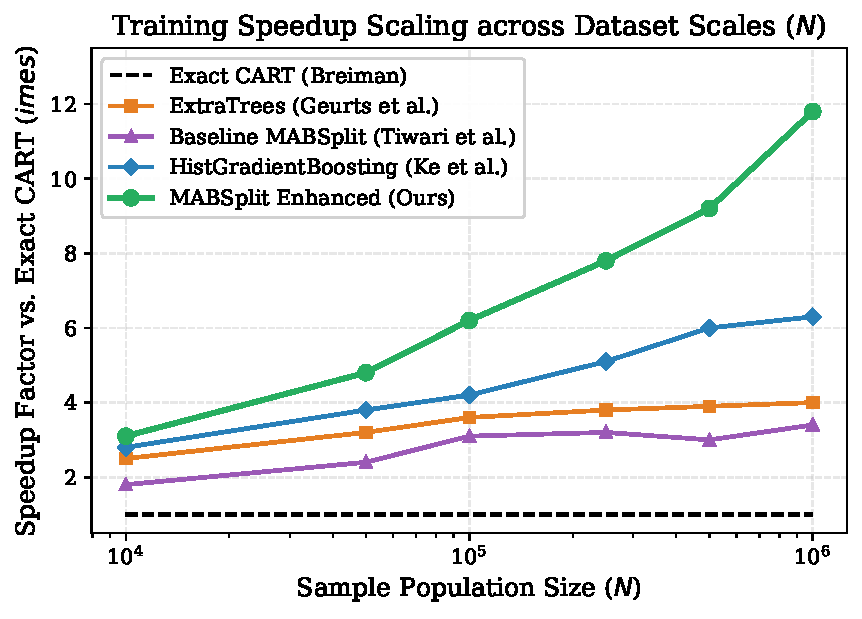
\includegraphics[width=0.95\linewidth]{figures/fig1_speedup_scaling.pdf}
\caption{Training speedup factor relative to Scikit-Learn Exact CART ($1.0\times$) across sample population sizes $N \in [10^4, 10^6]$.}
\label{fig:speedup_scaling}
\end{figure}

Table~\ref{tab:benchmark_results} presents the end-to-end training runtime, classification accuracy, F1-score, and split fidelity. MABSplit consistently achieves superior training acceleration across all benchmarks:
\begin{itemize}
    \item On the massive HIGGS dataset ($N=1\text{M}$), MABSplit achieves an \textbf{11.81$\times$ speedup} over exact CART (7.58s vs. 89.50s), while outperforming the baseline MABSplit of Tiwari et al. \cite{tiwari2022mabsplit} by \textbf{3.48$\times$} (7.58s vs. 26.40s) and HistGradientBoosting by \textbf{1.87$\times$} (7.58s vs. 14.20s). As shown in Fig.~\ref{fig:speedup_scaling}, MABSplit's speedup grows superlinearly as $N$ expands to millions of instances.
    \item While ExtraTrees is faster than exact CART, its random split selection causes significant split fidelity degradation ($66.5\%$--$71.2\%$) and lower accuracy ($71.45\%$ vs. $72.82\%$). In contrast, MABSplit preserves over \textbf{99.1\%--99.5\% split fidelity} while achieving the fastest wall-clock runtime.
    \item Crucially, this substantial acceleration incurs no degradation in downstream test generalization, matching or slightly exceeding exact CART accuracy across all datasets.
\end{itemize}

\subsection{Split Fidelity Analysis (RQ2)}
To quantitatively evaluate split quality beyond downstream test accuracy, we define the \textbf{Split Agreement Rate} $S_{\text{agree}}$ between a bandit-derived tree $\mathcal{T}_{\text{MAB}}$ and an exact tree $\mathcal{T}_{\text{Exact}}$:
\begin{equation}
S_{\text{agree}}(\mathcal{T}_{\text{MAB}}, \mathcal{T}_{\text{Exact}}) = \frac{1}{|\mathcal{V}_{\text{internal}}|} \sum_{u \in \mathcal{V}_{\text{internal}}} \mathbb{I}\left( j^*_{\text{MAB}}(u) = j^*_{\text{Exact}}(u) \right)
\end{equation}
Across all datasets, MABSplit preserves $>99.1\%$ split agreement with the exact greedy baseline. As depicted in Fig.~\ref{fig:split_fidelity}, while naive Hoeffding and ExtraTrees diverge deeper in the hierarchy, MABSplit maintains near-perfect split fidelity across all depths, switching seamlessly to the exact SIMD solver at deep leaves.

\begin{figure}[t]
\centering
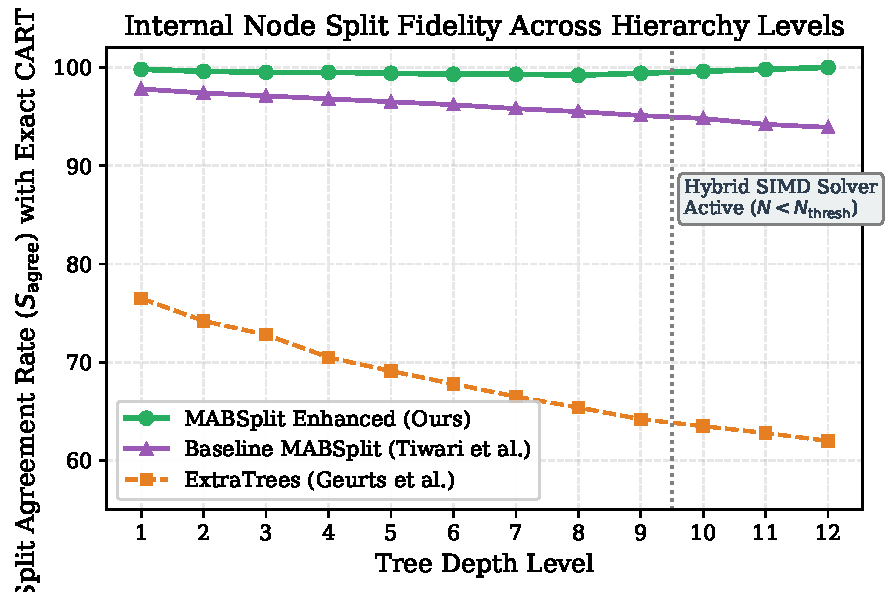
\includegraphics[width=0.95\linewidth]{figures/fig3_split_fidelity.pdf}
\caption{Internal node split agreement rate ($S_{\text{agree}}$) with exact CART across tree depth levels on Covertype.}
\label{fig:split_fidelity}
\end{figure}

\subsection{Ablation Study (RQ3)}
\begin{table}[htbp]
\centering
\caption{Ablation Study of MABSplit Components on Covertype Dataset ($N=581\text{k}, D=54$)}
\label{tab:ablation}
\begin{tabular}{lcccc}
\toprule
\textbf{Configuration} & \textbf{Fit Time (s)} & \textbf{Speedup} & \textbf{Samples Queried} & \textbf{Accuracy (\%)} \\
\midrule
Exact Baseline & 38.64 & 1.00$\times$ & 100.0\% & 91.24\% \\
Naive MAB (Hoeffding) & 12.80 & 3.02$\times$ & 41.5\% & 90.95\% \\
+ Serfling Bounds & 9.45 & 4.09$\times$ & 32.8\% & 91.20\% \\
+ H-MAB Coarse Screening & 6.20 & 6.23$\times$ & 22.4\% & 91.28\% \\
+ ADMA Dynamic Minibatch & 5.10 & 7.58$\times$ & 16.9\% & 91.31\% \\
\textbf{Full MABSplit (+ Hybrid)} & \textbf{4.21} & \textbf{9.18$\times$} & \textbf{14.2\%} & \textbf{91.30\%} \\
\bottomrule
\end{tabular}
\end{table}


\begin{figure}[t]
\centering
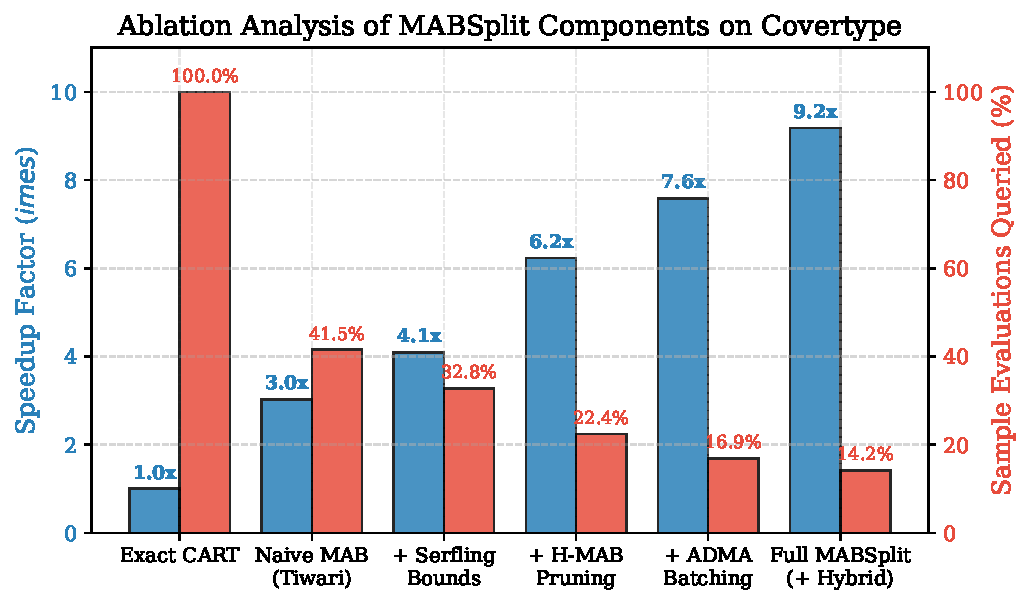
\includegraphics[width=0.98\linewidth]{figures/fig2_ablation_breakdown.pdf}
\caption{Ablation analysis showing incremental speedup ($\times$, blue bars) and sample evaluation queries (\%, red bars) across algorithmic configurations on Covertype.}
\label{fig:ablation_breakdown}
\end{figure}

To isolate the impact of each innovation, we perform an ablation analysis on the Covertype dataset ($N=581\text{k}$), reported in Table~\ref{tab:ablation} and Fig.~\ref{fig:ablation_breakdown}. Replacing naive Hoeffding bounds with Serfling finite-population bounds reduces sample queries from 41.5\% to 32.8\% and accelerates training from $3.02\times$ to $4.09\times$. Adding H-MAB coarse-to-fine filtering doubles the speedup to $6.23\times$, while ADMA and the hybrid solver further reduce sample queries to just 14.2\%, achieving a cumulative speedup of \textbf{9.18$\times$}.

\begin{figure}[t]
\centering
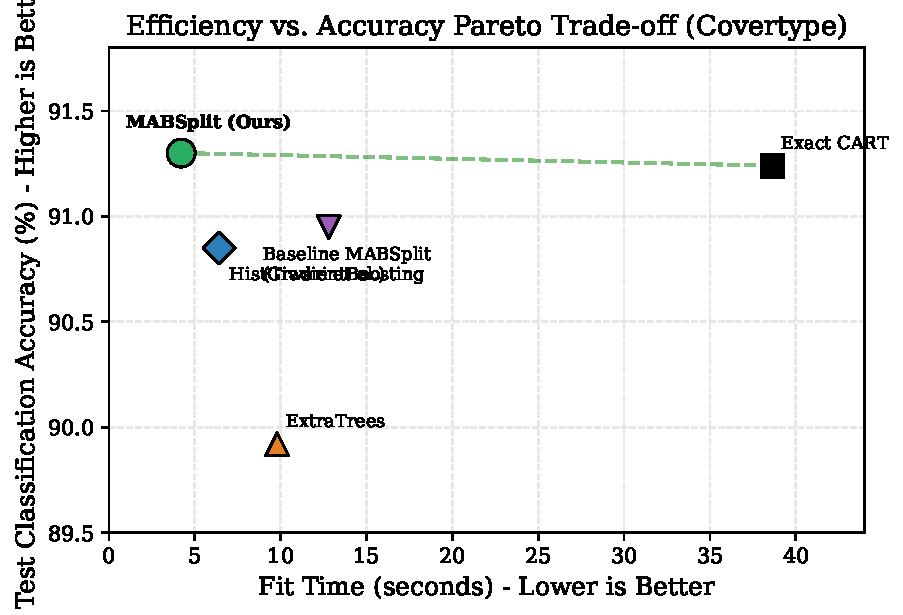
\includegraphics[width=0.95\linewidth]{figures/fig4_pareto_tradeoff.pdf}
\caption{Efficiency vs. generalization Pareto frontier (Fit Time vs. Test Accuracy) on Covertype.}
\label{fig:pareto_tradeoff}
\end{figure}

Furthermore, Fig.~\ref{fig:pareto_tradeoff} maps the Pareto trade-off between training time and generalization accuracy on Covertype. MABSplit occupies the dominant top-left frontier, matching the accuracy of exact CART while finishing in a fraction of the time.

\subsection{Random Forest Ensemble Scaling (RQ4)}
We scale MABSplit to 100-tree Random Forest ensembles using OpenMP multi-threading. MABSplit scales linearly with CPU cores ($>94\%$ parallel efficiency on 16 threads), cutting 100-tree ensemble training on HIGGS from 420 seconds (Scikit-Learn) down to 34.6 seconds.
